% ^^A -*- japanese-latex -*-
%
% \ifx\epTeXinputencoding\undefined\else
%   \epTeXinputencoding utf8
% \fi
% \iffalse
%<*driver>
\ifx\epTeXinputencoding\undefined\else
  \epTeXinputencoding utf8
\fi
%</driver>
%
%   bellsmacros.dtx
%
%<*driver>
\documentclass[uplatex,a4paper,12Q,dvipdfmx]{jsarticle}
%\documentclass[lualatex,a4paper,12Q]{jlreq}
\usepackage{doc}
\usepackage{ifptex}
\ifptex
  \xspcode"5C=1 %% \
  \xspcode"22=1 %% "
\fi
\addtolength{\textwidth}{-1in}
\addtolength{\evensidemargin}{1in}
\addtolength{\oddsidemargin}{1in}
\addtolength{\marginparwidth}{1in}
\setlength\marginparpush{0pt}
\usepackage{etoolbox}
% \usepackage{listings}
% \ifptex
%   \usepackage{jlisting}
% \fi
\usepackage{color}
\usepackage{xspace}
\usepackage{ifpdf}
\usepackage{hyperref}
\ifptex
  \usepackage{pxjahyper}
\fi
\usepackage[T1]{fontenc}
\usepackage{lmodern}
\definecolor{myblue}{rgb}{0,0,0.75}
\definecolor{mygreen}{rgb}{0,0.45,0}
\CodelineNumbered
\EnableCrossrefs
\CodelineIndex
\RecordChanges % Gather update information
\setcounter{StandardModuleDepth}{1}

\def\TikZ{Ti\textsl{k}Z}
\newcommand*{\Lcount}[1]{\textsl{\small#1}}
\newcommand*{\Lopt}[1]{\textsf{#1}}
\newcounter{@clineno}
\def\mlineplus#1{\setcounter{@clineno}{\arabic{CodelineNo}}%
   \addtocounter{@clineno}{#1}\arabic{@clineno}}
\makeatletter
\DeclareRobustCommand{\cmd}[1]{\cs{\expandafter\cmd@to@cs\string#1}}
\def\cmd@to@cs#1#2{\char\number`#2\relax}
\makeatother
\DeclareRobustCommand{\cs}[1]{\texttt{\char`\\#1}}
\providecommand{\marg}[1]{%
  {\ttfamily\char`\{}\meta{#1}{\ttfamily\char`\}}}
\providecommand{\oarg}[1]{%
  {\ttfamily[}\meta{#1}{\ttfamily]}}
\newrobustcmd*{\env}[1]{\mbox{\ttfamily#1}}
\newrobustcmd*{\file}[1]{\mbox{\ttfamily#1}}
\newrobustcmd*{\prm}[1]{
  \ifblank{#1}
    {}
    {\mbox{%
       \ensuremath\langle
       \normalfont\textit{#1}%
       \ensuremath\rangle}}}

\usepackage{bellsmacros}
\hypersetup{colorlinks,hyperfootnotes=false,linkcolor=myblue,urlcolor=mygreen}

\GetFileInfo{bellsmacros.sty}
\begin{document}
  \DocInput{bellsmacros.dtx}
\end{document}
%</driver>
%
% \fi
% \changes{v1.0}{2019/10/29}
%   {make this .dtx file}
% \def\Omaginai{依存パッケージ}
% \def\Ghost{ゴースト文字マクロの定義}
% \def\Constants{定数の定義}
% \def\Environments{環境定義}
% \def\Romans{ローマ数字}
% \def\Arrows{矢印など}
% \def\Mathematics{数学表記}
% \def\Underlines{\file{udline}関係}
% \def\Nihongo{日本語処理関係}
% \def\TikZMacros{\TikZ 関係}
% \def\Sakuin{索引関係}
% \def\Sanshou{参照関係}
% \def\DraftMacros{仮組み関係}
% \title{bellsmacros}
% \author{bell}
% \date{\filedate}
% \maketitle
% \tableofcontents
%
% \MakeShortVerb{\|}
%
% \section{はじめに}
% \iffalse \section{概要}
%
%
% \subsection{\Omaginai}
% \begin{itemize}
% \item \file{amsmath}
% \item \file{amssymb}
% \item \file{etoolbox}
% \item \file{framed}
% \item \file{mathtools}
% \item \file{theorem}
% \item \file{hyperref}
% \item \file{pxjahyper}
% \item \file{tikz}
% \item \file{udline}
% \item \file{makeidx}
% \end{itemize}
% \subsection{\Ghost}
% \DescribeMacro{\eghost}
% \DescribeMacro{\jghost}
% \cmd{\eghost}は英文ゴーストを, \cmd{\jghost}は和文ゴーストを作ります.
%
% \subsection{\Constants}
% 内部で使う定数を設定しています.
% 
% \subsection{\Environments}
% \subsubsection{\file{theorem}依存のもの}
% \subsubsection{非依存のもの}
% \subsubsection{\file{framed}依存のもの}
% \subsection{\Romans}
% 
% \subsection{\Arrows}
% 
% \subsection{\Mathematics}
% 
% \subsection{\Underlines}
% \subsection{\Nihongo}
% 
% \subsection{\TikZMacros}
% 
% \subsection{\Sakuin}
% 
% \subsection{\Sanshou}
% \subsubsection{非依存のもの}
% \subsubsection{\file{mathtools}依存のもの}
% 
% \subsection{\DraftMacros}
% \fi
% \StopEventually{}
% \section{実装}
%    \begin{macrocode}
%<*bellsmacros>
%%============================================================================%%
%%                                                                            %%
%%   M         M      A         CCCCC     RRRRRRR      OOOOO      SSSSS       %%
%%   MM       MM     A A       C     C    R      R    O     O    S     S      %%
%%   M M     M M    A   A     C       C   R       R  O       O  S       S     %%
%%   M M     M M   A     A    C           R       R  O       O   SS           %%
%%   M  M   M  M  A       A   C           RRRRRRRR   O       O     SSS        %%
%%   M  M   M  M  AAAAAAAAA   C           R      R   O       O        SS      %%
%%   M   M M   M  A       A   C       C   R       R  O       O  S       S     %%
%%   M   M M   M  A       A    C     C    R       R   O     O    S     S      %%
%%   M    M    M  A       A     CCCCC     R       R    OOOOO      SSSSS       %%
%%                                                                            %%
%%============================================================================%%
% \NeedsTeXFormat{pLaTeX2e}
\NeedsTeXFormat{LaTeX2e}
\ProvidesPackage{bellsmacros}
  [2020/01/25 bell's (up)LaTeX macro set]
% [2019/11/04 bell's (up)LaTeX macro set]
%    \end{macrocode}
% \subsection{\Omaginai}
%    \begin{macrocode}
%%==============================================================================
%% 依存パッケージの読み込み
%%==============================================================================
\RequirePackage{amsmath}
\RequirePackage{amssymb}
%\RequirePackage{amsthm}
\RequirePackage{etoolbox}
\RequirePackage{framed}
\RequirePackage{ifptex}
\RequirePackage{mathtools}
\RequirePackage{theorem}
\RequirePackage{hyperref}
\hypersetup{hidelinks=true}
\ifptex
  \RequirePackage{pxjahyper}
\fi
% \RequirePackage{pxghost}
\RequirePackage{bxghost}
% \RequirePackage{pgfmath}
\RequirePackage{tikz}
\usetikzlibrary{calc,positioning,quotes}
\RequirePackage{udline}
\RequirePackage{makeidx}


%    \end{macrocode}
% \subsection{\Ghost}
%    \begin{macrocode}
%%==============================================================================
%% ゴースト文字マクロの定義(bxghost依存)
%%==============================================================================
%    \end{macrocode}
%    \begin{macrocode}
\def\eghost{\eghostguarded{}}
%    \end{macrocode}
%    \begin{macrocode}
\def\jghost{\jghostguarded{}}
%    \end{macrocode}
%    \begin{macrocode}
%%==============================================================================
%% 定数の定義
%%==============================================================================
%    \end{macrocode}
% \subsection{\Constants}
%    \begin{macrocode}
\newlength\bellTempdima
\newlength\bellTempdimb
\newif\if@DEBUG%for debuging only

\def\@to{to}
\def\p@ne{.1}
\def\qu@rt{.25}
\def\h@lf{.5}
\def\p@seven{.7}
\def\thr@@qu@rt{.75}

\chardef\f@ur=4
\chardef\fiv@=5
\chardef\si@=6
\chardef\s@v@n=7
\chardef\@ight=8
\chardef\nin@=9
\chardef\t@n=10
\chardef\@l@v@n=11
\chardef\tw@lv@=12
\chardef\fourt@@n=14
\chardef\fiv@t@@n=15
\chardef\tw@nty=20
\chardef\@xxiii=23
\chardef\@xxv=25
\chardef\@xxiv=24
\chardef\@xxvi=26
\chardef\@xxvii=27
\chardef\@xxix=29
\chardef\@xxxii=32
\chardef\@xl=40
\chardef\@xli=41
\chardef\@xlv=45
\chardef\@l=50
\chardef\@lii=52
\chardef\@liv=54
\chardef\@lxxxiii=83
\chardef\@c=100
\chardef\@cxv=115
\chardef\@cxxviii=128

\ifptex
  \def\bell@zw{zw}
  \def\bell@zh{zh}
\else
  \ifdefined\zw \let\bell@zw\zw
  \else
    \PackageError
      {bellsmacros}%
      {\noexpand\zw\space has no reasonable meaning.}%
      {Load luatex-ja (if you using lualatex) before loading this
       or use (u)pTeX.}%
  \fi
  \ifdefined\zh \let\bell@zh\zh
  \else
    \PackageError
      {bellsmacros}
      {\noexpand\zh\space has no reasonable meaning.}
      {Load luatex-ja (if you using lualatex) before loading this
       or use (u)pTeX.}%
  \fi
\fi
%    \end{macrocode}
% \subsection{\Environments}
% \subsubsection{\file{theorem}依存のもの}
%    \begin{macrocode}
%%==============================================================================
%% 環境定義(theorem依存)
%%==============================================================================
%    \end{macrocode}
%    \begin{macrocode}
\theorembodyfont{\normalfont}
\theoremstyle{break}
\newtheorem{@theory}{定理}
\newtheorem{@definition}{定義}
\newtheorem{@lemma}{補題}
\theorempreskipamount\z@
\theorempostskipamount\z@

\newenvironment{theory}
  {\begin{oframed}\begin{@theory}}
  {\end{@theory}\end{oframed}}
\newenvironment{definition}
  {\begin{oframed}\begin{@definition}}
  {\end{@definition}\end{oframed}}
\newenvironment{lemma}
  {\begin{oframed}\begin{@lemma}}
  {\end{@lemma}\end{oframed}}
\let\defi\definition
\let\enddefi\enddefinition
\let\theo\theory
\let\endtheo\endtheory
\let\theorem\theory
\let\endtheorem\endtheory

%    \end{macrocode}
% \subsubsection{非依存のもの}
%    \begin{macrocode}
%%==============================================================================
%% 環境定義
%%==============================================================================
%    \end{macrocode}
%    \begin{macrocode}
\def\bell@envtemplate{%
  \setlength{\topsep}{\qu@rt\baselineskip}%
  \setlength{\listparindent}{1\bell@zw}%
  \settowidth{\labelwidth}{\@itemlabel}%
  \divide\labelwidth\dimexpr1\bell@zw\relax
  \multiply\labelwidth\dimexpr1\bell@zw\relax
  \setlength{\itemindent}{\labelwidth}%
  \addtolength{\itemindent}{\h@lf\listparindent}%
  \setlength{\labelsep}{\h@lf\listparindent}%
}

%    \end{macrocode}
%    \begin{macrocode}
\newenvironment{setsumei}{%
  \begin{list}{\textgt{\inhibitglue [説明]}}{%
  \setlength{\leftmargin}{2\bell@zw}%
  \bell@envtemplate
  \setlength{\rightmargin}{0\bell@zw}%
  }%
  \item}{\vspace{-\h@lf\topsep}\end{list}%
}

%    \end{macrocode}
%    \begin{macrocode}
\newenvironment{NB}{%
  \begingroup\par\begin{list}{N.B.}{%
  \setlength{\leftmargin}{2\bell@zw}%
  \small%
  \bell@envtemplate
  \setlength{\rightmargin}{\leftmargin}%
  }%
  \item}{\vspace{-\h@lf\topsep}\end{list}\endgroup%
}

%    \end{macrocode}
%    \begin{macrocode}
\newenvironment{chuui}{%
  \begingroup\par\begin{list}{\inhibitglue \textgt{[注意]}}{%
  \setlength{\leftmargin}{2\bell@zw}%
  \small%
  \bell@envtemplate
  \setlength{\rightmargin}{\leftmargin}%
  }%
  \item}{\vspace{-\h@lf\topsep}\end{list}\endgroup%
}

%    \end{macrocode}
%    \begin{macrocode}
\newenvironment{proof}{%
  \begin{list}{\textgt{\inhibitglue [証明]}}{%
  \setlength{\leftmargin}{1\bell@zw}%
  \bell@envtemplate
  }\begin{proofleftbar}%
  \item}{\end{proofleftbar}\vspace{\h@lf\topsep}\end{list}%
}

%    \end{macrocode}
%    \begin{macrocode}
\newenvironment{Yodan}{%
  \begingroup\par\begin{list}{\textgt{\inhibitglue [余談]}}{%
  \setlength{\leftmargin}{2\bell@zw}%
  \small%
  \bell@envtemplate
  \setlength{\rightmargin}{\leftmargin}%
  }%
  \item}{\vspace{-\h@lf\topsep}\end{list}\endgroup%
}

%    \end{macrocode}
%    \begin{macrocode}
\def\FGNsize{\small}
\def\@FGN{%
  \setlength{\leftmargin}{2\bell@zw}%
  \FGNsize
  \bell@envtemplate
  \setlength{\rightmargin}{\leftmargin}%
}

%    \end{macrocode}
%    \begin{macrocode}
\newenvironment{FGN}{%
  \begingroup\par\begin{list}{\textgt{\inhibitglue [附言]}}{\@FGN}%
  \item}{\vspace{-\h@lf\topsep}\end{list}\endgroup%
}

%    \end{macrocode}
%    \begin{macrocode}
\newcounter{FGNenumi}[subsection]
\renewcommand{\theFGNenumi}{[附言\Roman{FGNenumi}]}
\newenvironment{FGNenum}[1][-1]{%
  \ifnum #1<\z@ \else \setcounter{FGNenumi}{#1}\fi
  \refstepcounter{FGNenumi}\par\vspace{.3\bell@zh}%
  \begin{list}{\textgt{\inhibitglue\theFGNenumi}}{\@FGN}%
  \item}{\vspace{-\h@lf\topsep}\end{list}%
}

\newcommand{\FGNlabel}[1]{\label{FGN:#1}}
\newcommand{\FGNref}[1]{\ref{FGN:#1}}

%    \end{macrocode}
%    \begin{macrocode}
%%==============================================================================
%% 環境定義(framed依存)
%%==============================================================================
%    \end{macrocode}
%    \begin{macrocode}
\newcounter{exampleNumber}
\def\theexampleNumber{例\arabic{exampleNumber}.}
\newenvironment{example}[1][]{%
  \begin{oframed}
  \def\reseaved@a{#1}%
  \begin{list}
  {\theexampleNumber\ifx\reseaved@a\empty
    \else [\headfont{#1}]\fi}%
  {\setlength{\leftmargin}{1.5\bell@zw}%
  \setlength{\rightmargin}{0\bell@zw}%
  \small%
  \setlength{\listparindent}{1\bell@zw}%
  \settowidth{\labelwidth}{\@itemlabel}%
  \setlength{\itemindent}{\labelwidth}%
  \addtolength{\itemindent}{\h@lf\listparindent}%
  \setlength{\labelsep}{\h@lf\listparindent}%
  \refstepcounter{exampleNumber}}%
  \item}{\end{list}\end{oframed}%
}
\let\EG\example
\let\endEG\endexample


\newenvironment{proofleftbar}{%
  \def\FrameCommand{\hspace{1\bell@zw}\vrule\@width2pt\kern-2pt\relax}% 
  \MakeFramed {\advance\hsize-\width \FrameRestore}}%
  {\endMakeFramed}

\renewenvironment{framed}% using default \FrameCommand
  {\MakeFramed{\advance\hsize-\width \FrameRestore}}%
  {\endMakeFramed}

%    \end{macrocode}
% \subsection{\Romans}
%    \begin{macrocode}
%%==============================================================================
%% ローマ数字(hyperref依存)
%%==============================================================================
%    \end{macrocode}
%    \begin{macrocode}
\DeclareRobustCommand{\Greak@Numberbox}[2]
  {\texorpdfstring{\eghostguarded{#1}}{#2}}
\DeclareRobustCommand{\Gni}
  {\Greak@Numberbox{\textrm{I}}{I}}
\DeclareRobustCommand{\Gnii}
  {\Greak@Numberbox{\textrm{I\nobreak\hspace{-0.1em}I}}
                   {II}}
\DeclareRobustCommand{\Gniii}
  {\Greak@Numberbox{\textrm{I\nobreak\hspace{-0.1em}I\nobreak\hspace{-0.1em}I}}
                   {III}}
\DeclareRobustCommand{\Gniv}
  {\Greak@Numberbox{\textrm{I\nobreak\hspace{-0.1em}V}}
                   {IV}}
\DeclareRobustCommand{\Gnv} 
  {\Greak@Numberbox{\textrm{V}}
                   {V}}
\DeclareRobustCommand{\Gnvi}
  {\Greak@Numberbox{\textrm{V\nobreak\hspace{-0.1em}I}}
                   {VI}}
\DeclareRobustCommand{\Gnvii}
  {\Greak@Numberbox{\textrm{V\nobreak\hspace{-0.1em}I\nobreak\hspace{-0.1em}I}}
                   {VII}}
\DeclareRobustCommand{\Gnviii}
  {\Greak@Numberbox{\textrm{V\nobreak\hspace{-0.1em}I\nobreak\hspace{-0.1em}I%
                              \nobreak\hspace{-0.1em}I}}
                   {VIII}}
\DeclareRobustCommand{\Gnix}
  {\Greak@Numberbox{\textrm{I\nobreak\hspace{-0.1em}X}}
                   {IX}}
\DeclareRobustCommand{\Gnx} 
  {\Greak@Numberbox{\textrm{X}}
                   {X}}
\DeclareRobustCommand{\Gnxi}
  {\Greak@Numberbox{\textrm{X\nobreak\hspace{-0.1em}I}}
                   {XI}}
\DeclareRobustCommand{\Gnxii}
  {\Greak@Numberbox{\textrm{X\nobreak\hspace{-0.1em}I\nobreak\hspace{-0.1em}I}}
                   {XII}}

\DeclareRobustCommand{\gni}
  {\Greak@Numberbox{\textrm{i}}
                   {i}}
\DeclareRobustCommand{\gnii}
  {\Greak@Numberbox{\textrm{i\nobreak\hspace{-0.1em}i}}
                   {ii}}
\DeclareRobustCommand{\gniii}
  {\Greak@Numberbox{\textrm{i\nobreak\hspace{-0.1em}i\nobreak\hspace{-0.1em}i}}
                   {iii}}
\DeclareRobustCommand{\gniv}
  {\Greak@Numberbox{\textrm{i\nobreak\hspace{-0.1em}v}}
                   {iv}}
\DeclareRobustCommand{\gnv}
  {\Greak@Numberbox{\textrm{v}}
                   {v}}
\DeclareRobustCommand{\gnvi}
  {\Greak@Numberbox{\textrm{v\nobreak\hspace{-0.1em}i}}
                   {vi}}
\DeclareRobustCommand{\gnvii}
  {\Greak@Numberbox{\textrm{v\nobreak\hspace{-0.1em}i\nobreak\hspace{-0.1em}i}}
                   {vii}}
\DeclareRobustCommand{\gnviii}
  {\Greak@Numberbox{\textrm{v\nobreak\hspace{-0.1em}i\nobreak\hspace{-0.1em}i%
                              \nobreak\hspace{-0.1em}i}}
                   {viii}}
\DeclareRobustCommand{\gnix}
  {\Greak@Numberbox{\textrm{i\nobreak\hspace{-0.1em}x}}
                   {ix}}
\DeclareRobustCommand{\gnx}
  {\Greak@Numberbox{\textrm{x}}
                   {x}}
\DeclareRobustCommand{\gnxi}
  {\Greak@Numberbox{\textrm{x\nobreak\hspace{-0.1em}i}}
                   {xi}}
\DeclareRobustCommand{\gnxii}
  {\Greak@Numberbox{\textrm{x\nobreak\hspace{-0.1em}i\nobreak\hspace{-0.1em}i}}
                   {xii}}

%    \end{macrocode}
% \subsection{\Arrows}
%    \begin{macrocode}
%%==============================================================================
%% 矢印など
%%==============================================================================
%    \end{macrocode}
%    \begin{macrocode}
\newcommand{\Arrowright}{%
  \ensuremath{\rightarrow}%
}
\newcommand{\Arrowleft}{%
  \ensuremath{\leftarrow}%
}
\newcommand{\Arrowleftright}{%
  \ensuremath{\leftrightarrow}%
}
\newcommand{\Arrowdown}{%
  \ensuremath{\downarrow}%
}
\newcommand{\Arrowup}{%
  \ensuremath{\uparrow}%
}
\newcommand{\Cross}{%
  \ensuremath{\times}%
}

%    \end{macrocode}
% \subsection{\Mathematics}
%    \begin{macrocode}
%%==============================================================================
%% 数学表記(amsmath依存)
%%==============================================================================
%    \end{macrocode}
% \begin{macro}{\comp}
% 複素数(complex number)全体の成す集合$\comp$を出力します.
%    \begin{macrocode}
\newcommand{\comp}{\mathbf C}% 複素数
%    \end{macrocode}
% \end{macro}
% \begin{macro}{\real}
% 実数(real number)全体の成す集合$\real$を出力します.
%    \begin{macrocode}
\newcommand{\real}{\mathbf R}% 実数
%    \end{macrocode}
% \end{macro}
% \begin{macro}{\zahl}
% 整数(Ger: Ganze Zahl)全体の成す集合$\zahl$を出力します.
%    \begin{macrocode}
\newcommand{\zahl}{\mathbf Z}% 整数
%    \end{macrocode}
% \end{macro}
% \begin{macro}{\numb}
% 自然数(natural number)全体の成す集合$\numb$を出力します.
%    \begin{macrocode}
\newcommand{\numb}{\mathbf N}% 自然数

%    \end{macrocode}
% \end{macro}
% \begin{macro}{\re}
% 複素数の実部を示す$\re$を出力します.
%    \begin{macrocode}
\newcommand{\re}{\mathfrak{Re}}% 実部
%    \end{macrocode}
% \end{macro}
% \begin{macro}{\im}
% 複素数の虚部を示す$\im$を出力します.
%    \begin{macrocode}
\newcommand{\im}{\mathfrak{Im}}% 虚部

%    \end{macrocode}
% \end{macro}
% \begin{macro}{\mhyphen}
% 数式環境内でハイフン$\mhyphen$を出力します.
%    \begin{macrocode}
\mathchardef\mhyphen="2D% Hyphen
%    \end{macrocode}
% \end{macro}
% \begin{macro}{\minfty}
% 負の無限大$\minfty$を出力します.
%    \begin{macrocode}
\newcommand{\minfty}{{-\infty}}% 負の無限大

%    \end{macrocode}
% \end{macro}
% \begin{macro}{\Res}
%    \begin{macrocode}
\newcommand{\Res}{\mathop{\operator@font Res}}% 留数
%    \end{macrocode}
% \end{macro}
% \begin{macro}{\Hom}
%    \begin{macrocode}
\newcommand{\Hom}{\mathop{\operator@font Hom}}% 準同型写像

%    \end{macrocode}
% \end{macro}
% \begin{macro}{\norm}
%    \begin{macrocode}
\def\norm#1{\left\lVert#1\right\rVert}% ノルム
%    \end{macrocode}
% \end{macro}
% \begin{macro}{\abs}
%    \begin{macrocode}
\def\abs#1{\left\lvert#1\right\rvert}% 絶対値
\let\Abs\abs

%    \end{macrocode}
% \end{macro}
% \begin{macro}{\bell@diff}
%    \begin{macrocode}
\def\bell@diff#1{\mathrm{d}#1\ }
%    \end{macrocode}
% \end{macro}
% \begin{macro}{\bell@sdiff}
%    \begin{macrocode}
\def\bell@sdiff#1{\mathrm{d}#1}
%    \end{macrocode}
% \end{macro}
% \begin{macro}{\diff}
%    \begin{macrocode}
\newcommand{\diff}{\@ifstar{\bell@sdiff}{\bell@diff}}% 微分のd

%    \end{macrocode}
% \end{macro}
% \begin{macro}{\bell@pdiff}
%    \begin{macrocode}
\def\bell@pdiff#1{\partial#1\ }
%    \end{macrocode}
% \end{macro}
% \begin{macro}{\bell@spdiff}
%    \begin{macrocode}
\def\bell@spdiff#1{\partial#1}
%    \end{macrocode}
% \end{macro}
% \begin{macro}{\pdiff}
%    \begin{macrocode}
\newcommand{\pdiff}{\@ifstar{\bell@spdiff}{\bell@pdiff}}% 偏微分の∂

%    \end{macrocode}
% \end{macro}
% \begin{macro}{\dif}
%    \begin{macrocode}
\newcommand{\dif}[2][]{\frac{\mathrm d#1}{\mathrm d#2}}% 一階微分
%    \end{macrocode}
% \end{macro}
% \begin{macro}{\ddif}
%    \begin{macrocode}
\newcommand{\ddif}[2][]{\frac{\mathrm d^2#1}{\mathrm d#2^2}}% 二階微分
%    \end{macrocode}
% \end{macro}
% \begin{macro}{\pdif}
%    \begin{macrocode}
\newcommand{\pdif}[2][]{\frac{\partial#1}{\partial#2}}% 一階偏微分
%    \end{macrocode}
% \end{macro}
% \begin{macro}{\pddif}
%    \begin{macrocode}
\newcommand{\pddif}[2][]{\frac{\partial^2 #1}{\partial #2^2}}% 二階偏微分

%    \end{macrocode}
% \end{macro}
% \begin{macro}{\bell@differentialOP}
%    \begin{macrocode}
\def\bell@differentialOP#1[#2]#3{%
  \frac{\mathrm d^{#1}#2}{\mathrm d#3^{#1}}}
%    \end{macrocode}
% \end{macro}
% \begin{macro}{\bell@partialderivativeOP}
%    \begin{macrocode}
\def\bell@partialderivativeOP#1[#2]#3{%
  \frac{\partial^{#1}#2}{\partial #3^{#1}}}
%    \end{macrocode}
% \end{macro}
% \begin{macro}{\ndif}
%    \begin{macrocode}
\newcommand{\ndif}[1]{%
  \@ifnextchar[{\bell@differentialOP{#1}}%
               {\bell@differentialOP{#1}[]}}% n階微分
%    \end{macrocode}
% \end{macro}
% \begin{macro}{\npdif}
%    \begin{macrocode}
\newcommand{\npdif}[1]{%
  \@ifnextchar[{\bell@partialderivativeOP{#1}}%
               {\bell@partialderivativeOP{#1}[]}}% n階偏微分

%    \end{macrocode}
% \end{macro}
% \begin{macro}{\Fourier}
%    \begin{macrocode}
\newcommand{\Fourier}{\mathcal{F}}% Fourier変換演算子
%    \end{macrocode}
% \end{macro}
% \begin{macro}{\Laplace}
%    \begin{macrocode}
\newcommand{\Laplace}{\mathcal{L}}% Laplace変換演算子

%    \end{macrocode}
% \end{macro}
% \begin{macro}{\sinc}
%    \begin{macrocode}
\newcommand{\sinc}{\mathrm{sinc}~}% sinc関数
%    \end{macrocode}
% \end{macro}
% \begin{macro}{\mathbfit}
%    \begin{macrocode}
\newcommand{\mathbfit}{\boldsymbol}% 太字斜体
\let\mathitbf\mathbfit% 太字斜体

%    \end{macrocode}
% \end{macro}
% \begin{macro}{\f@tok}
%    \begin{macrocode}
\ifx\f@tok\@undefined
\def\f@tok#1#2\af@tok{#1}
\fi
%    \end{macrocode}
% \end{macro}
% \begin{macro}{\tatev}
%    \begin{macrocode}
\def\tatev#1{%
  \displaystyle\begin{pmatrix}\bell@tatev#1;\relax;\end{pmatrix}}% 縦ベクトル
%    \end{macrocode}
% \end{macro}
% \begin{macro}{\bell@tatev}
%    \begin{macrocode}
\def\bell@tatev#1;#2;{%
  \def\reserved@a{#1}\def\reserved@b{#2}\reserved@a
    \expandafter\expandafter\expandafter
    \ifx\expandafter\f@tok\reserved@b\af@tok\relax
    \let\n@xt\relax
  \else
    \\%
    \let\n@xt\bell@tatev\def\reserved@b{#2;}%
  \fi
  \expandafter\n@xt\reserved@b%
}%
%    \end{macrocode}
% \end{macro}
% \begin{macro}{\yokov}
%    \begin{macrocode}
\def\yokov#1{%
  \displaystyle\begin{pmatrix}\bell@yokov#1;\relax;\end{pmatrix}}% 横ベクトル
%    \end{macrocode}
% \end{macro}
% \begin{macro}{\bell@yokov}
%    \begin{macrocode}
\def\bell@yokov#1;#2;{%
  \def\reserved@a{#1}\def\reserved@b{#2}\def\reserved@c{&}\reserved@a
  \expandafter\expandafter\expandafter
  \ifx\expandafter\f@tok\reserved@b\af@tok\relax
    \let\n@xt\relax
  \else
    \reserved@c%
    \let\n@xt\bell@yokov\def\reserved@b{#2;}%
  \fi
  \expandafter\n@xt\reserved@b%
}%
%    \end{macrocode}
% \end{macro}
% \begin{macro}{\Matrix}
%    \begin{macrocode}
\def\Matrix#1{\displaystyle\begin{pmatrix}#1\end{pmatrix}}% 行列

%    \end{macrocode}
% \end{macro}
% \subsection{\Underlines}
%    \begin{macrocode}
%%==============================================================================
%% udline関係
%%==============================================================================
%    \end{macrocode}
%    \begin{macrocode}
\setulminsep{0.55ex}{0.55ex}
\setulsep{0.0ex}
%    \end{macrocode}
% \subsection{\Nihongo}
%    \begin{macrocode}
%%==============================================================================
%% 日本語処理関係
%%==============================================================================
%    \end{macrocode}
%    \begin{macrocode}
\def\Qaki#1{\kern.25\bell@zw\<#1\kern.25\bell@zw\<}%両端に四分アキを入れる.
\def\xkanjispace{\kern\xkanjiskip}% 和欧文間グルーを入れる.
\def\Qspace#1{\kern#1\dimexpr.25\bell@zw\relax}% #1 Q幅のスペースを入れる.

%    \end{macrocode}
% \subsection{\TikZMacros}
%    \begin{macrocode}
%%==============================================================================
%% Tikz関係
%%==============================================================================
%    \end{macrocode}
%    \begin{macrocode}
\newcommand{\includeTikZpicture}[1]
  {\def\includeTikzPicture{true}\input{#1.tkz}\let\@includetikzpicture\relax}

%    \end{macrocode}
% \subsection{\Sakuin}
%    \begin{macrocode}
%%==============================================================================
%% 索引関係
%%==============================================================================
%    \end{macrocode}
%    \begin{macrocode}
\renewcommand{\seename}{\Arrowright}
\renewcommand*{\see}[2]{\seename #1}
\renewcommand{\alsoname}{参照}
%\let\Keyword\unl
\def\Keyword{\textbf}
% #1=別名(option), #2=キーワード
% 星付き: 強調表示せず
\DeclareRobustCommand{\KeyBF}
  {\@ifstar{\bell@KeyBFs}{\bell@KeyBF}}
\DeclareRobustCommand{\bell@KeyBF}[2][\relax]
  {\Keyword{#2}\ifx#1\relax\index{#2}\else\index{#2|see{#1}}\fi}
\DeclareRobustCommand{\bell@KeyBFs}[2][\relax]
  {#2\ifx#1\relax\index{#2}\else\index{#2|see{#1}}\fi}

%    \end{macrocode}
% \subsection{\Sanshou}
% \subsubsection{非依存のもの}
%    \begin{macrocode}
%%==============================================================================
%% 参照関係
%%==============================================================================
%    \end{macrocode}
%    \begin{macrocode}
\newcommand{\chapref}[1]  {\prechaptername\ref{chap:#1}\postchaptername}
\newcommand{\sectref}[1]  {\presectionname\ref{sect:#1}\postsectionname}
\newcommand{\ssectref}[1]  {\ref{ssect:#1}}
\newcommand{\sssectref}[1]  {\ref{sssect:#1}}
\newcommand{\figref}[1]    {\figurename \ref{fig:#1}}
\newcommand{\tblref}[1]    {\tablename \ref{tbl:#1}}
\ifdefined\eqref
  \let\bell@orig@eqref\eqref
  \renewrobustcmd{\eqref}[1]  {\bell@orig@eqref{eq:#1}}
\else
  \newrobustcmd{\eqref}[1]  {\ref{eq:#1}}
\fi
\newcommand{\chaplabel}[1]  {\label{chap:#1}}
\newcommand{\sectlabel}[1]  {\label{sect:#1}}
\newcommand{\ssectlabel}[1]  {\label{ssect:#1}}
\newcommand{\sssectlabel}[1]{\label{sssect:#1}}
\newcommand{\figlabel}[1]  {\label{fig:#1}}
\newcommand{\tbllabel}[1]  {\label{tbl:#1}}
\newcommand{\eqlabel}[1]  {\label{eq:#1}}

%    \end{macrocode}
% \subsubsection{\file{mathtools}依存のもの}
%    \begin{macrocode}
%%==============================================================================
%% 参照関係(mathtools依存)
%%==============================================================================
%    \end{macrocode}
%    \begin{macrocode}
\ifdefined\MHInternalSyntaxOn \MHInternalSyntaxOn
\def\MT_extended_eqref:n #1{
  \protected@write\@auxout{}
    {\string\MT@newlabel{eq:#1}}
  \textup{\let\df@label\@empty\MT_prev_tagform:n {\ref{eq:#1}}}
}
\EQ_MakeRobust\MT_extended_eqref:n
\renewcommand*\refeq[1]{
  \textup{\ref{eq:#1}}
}
\def\MT_extended_refeq:n #1{
  \protected@write\@auxout{}
    {\string\MT@newlabel{eq:#1}}
  \textup{\ref{eq:#1}}
}
\MHInternalSyntaxOff \fi

%    \end{macrocode}
% \subsection{\DraftMacros}
%    \begin{macrocode}
%%==============================================================================
%% 仮組み関係
%%==============================================================================
%    \end{macrocode}
%    \begin{macrocode}
\newcommand{\draftUC}{%
  \begin{figure}[H]\centering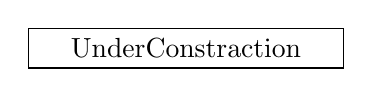
\begin{tikzpicture}
  \draw[semithick] (-2,0) rectangle (2,-.5);
  \node(UnderConstraction) at(0, 0)[below]{UnderConstraction};
  \end{tikzpicture}\end{figure}
}

\endinput
%    \end{macrocode}
%
% 以上で終わりです.
%
%    \begin{macrocode}
%</bellsmacros>
\endinput
%    \end{macrocode}
%
%
% \Finale
